\chapter{Church-Turing Tese}

De maskiner vi har kigget på indtil videre har enten været med endelig hukommelse (Endelige Automater) eller med en uendelig hukommelse der kun fungerer i en LIFO stak-hukommelse (PDA). Dermed er de for begrænset til at kunne agere som modeller af generelt-formåls computere, da disse har ubegrænset, uendelig hukommelse.

\section{Turingmaskiner}%
\label{sec:turingmachines}

I 1936 introducerede Alan Turing \textit{turingmaskinen}, en deterministisk model som minder om en endelig automat, men med uendeligt og ubegrænset hukommelse. Denne model af en maskine kan alt det som en almen computer\footnote{Her bruges ``almen computer'' som en oversættelse fra det engelske ``General Purpose Computer''} kan gøre. Dermed kan vi bruge denne model til at finde ud af begrænsninger m.m. om de computere vi bruger i dagligdagen.

En turingmaskine bruger et uendeligt bånd som dets hukommelse. Den har en \textit{båndhoved} som kan læse \textit{og skrive} symboler og flytte sig selv rundt på båndet. Til at starte med indeholder båndet kan input strengen, dog kan den skrive på dette bånd. Til at læse informationen går båndhovedet over de symboler der skal læses. Maskinen bliver ved med at komputere indtil den vælger at producere et output, enten \textit{accept} eller \textit{afvis}. Hvis den ikke kommer til et accept eller afvis state, så kører den for evigt, uden nogensinde at stoppe. Når komputeringen rammer en af disse states, stopper komputeringen.

\begin{figure}[ht]
	\centering
	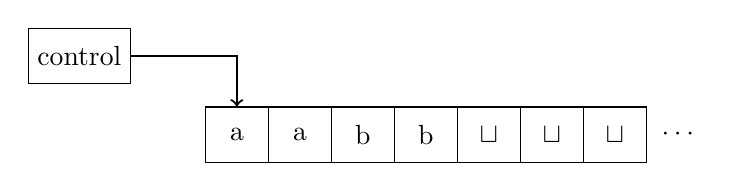
\begin{tikzpicture}
		\tikzset{block/.style={rectangle, draw, minimum height=2em, minimum width=3em}}
		\tikzset{line/.style={draw, -latex'}}
		\node[block] (control) {control};

		\node[block, minimum width=0.8cm] (a1) at (2,-1.0) {a};
		\node[block, minimum width=0.8cm] (a2) at (2.8,-1.0) {a};
		\node[block, minimum width=0.8cm] (b1) at (3.6,-1.0) {b};
		\node[block, minimum width=0.8cm] (b2) at (4.4,-1.0) {b};
		\node[block, minimum width=0.8cm] (b2) at (5.2,-1.0) {$\sqcup$};
		\node[block, minimum width=0.8cm] (b2) at (6.0,-1.0) {$\sqcup$};
		\node[block, minimum width=0.8cm] (b2) at (6.8,-1.0) {$\sqcup$};
		\node[label, minimum width=0.8cm] (b2) at (7.6,-1.0) {$\cdots$};

		\draw[->, thick] (control) -| (a1);
	\end{tikzpicture}
	\caption{\label{fig:turingschematic} Skematik af en turingmaskine.}
\end{figure}
I Figur~\ref{fig:turingschematic} kan der ses en skematik på en turingmaskine. Læg her mærke til at båndet er uendeligt langt, og efter input strengen er der bare blanke symboler, her betegnet som $\sqcup$.

Følgende punkter opsummerer forskellen mellem en endelig automat og en turingmaskine:

\begin{enumerate}
	\item En Turingmaskine kan både læse og skrive fra båndet.
	\item Læs-skriv (read-write) hovedet kan bevæge sig både til athøjre og til venstre.
	\item Båndet er uendeligt.
	\item De speceielle states til at acceptere og afvise et input træder i kraft med det samme.
\end{enumerate}



\subsection{Formel Definition af en Turingmaskine}%
\label{subsec:formaldefturingmachine}



Trods vi næsten aldrig bruger den formelle beskrivelse af en turingmaskine, da de oftest ender med at blive alt for store, giver vi den generelle formelle beskrivelse af en turingmaskine her.

Transitionsfunktionen i en turing maskine har formen $Q \times \Gamma \longrightarrow Q \times \Gamma \times \{L, R\}$. For eksempel betyder $\delta (q,a) = (r,b,L)$ at når båndet er over symbol $a$ og maskinen er i state $q$, så skal den skrive $b$ til symbolet hvor $a$ tidligere stod, og gå til state $r$. $L$ betyder her at den skal bevæge sig til venstre.

\begin{definition}[Formel Definition af en Turingmaskine]
	\label{def:formalturing}
	En \textbf{Turingmaskine} er en 7-tuple $(Q, \Sigma, \Gamma, \delta, q_{0}, q_{\text{accept}}, q_{\text{reject}})$, hvor $Q, \Sigma, \Gamma$ alle er endelige sæt, og
	\begin{enumerate}
		\item $Q$ er sættet af states.
		\item $\Sigma$ er inputalfabetet ikke indeholdende det blanke symbol, $\sqcup$.
		\item $\Gamma$ er båndalfabetet, hvor $\sqcup \in \Gamma$ og $\Sigma \subseteq \Gamma$.
		\item $\delta, Q \times \Gamma \longrightarrow Q \times \Gamma \times \{L, R\}$ er transitionsfunktionen.
		\item $q_{0} \in Q$ er startstaten.
		\item $q_{\text{accept}} \in Q$ er accept staten.
		\item $q_{\text{reject}} \in Q$ er afvis staten, hvor $q_{\text{accept}} \neq q_{\text{reject}}$.
	\end{enumerate}
\end{definition}

Bemærk at, på trods af at Sipser ikke skriver det som en mulighed, kan man nemt implementere ``stay'' (her skrevet S) som en mulighed, fromfor kun at vælge left eller right. Du kan gøre dette ved at først skrive, så gå til højre, så gå til venstre uden at gøre noget med symbolet.


\subsection{Turingmaskine Komputering}%
\label{subsec:turingmaskinekomputering}

En turingmaskine komputere ved at starte sit båndhoved på den venstremest symbol på båndet. Inputtet $w = w_{1}w_{2} \ldots w_{n} \in \Sigma^{*}$ er på de første (venstremest) $n$ pladser på båndet, og det resterende er blankt. Siden $\Sigma$ ikke indeholder de blanke symbol, kan man være sikker på at så snart det blanke symbol kommer på båndet, har man læst inputtet færdigt. Hvis hovedet nogensinde forsøger at bevæge sig mere til venstre end muligt, så forbliver hovedet på den venstremest symbolplacering, trods den ``skal'' gå til venstre. Når $M$ er begyndt bevæger den sig efter reglerne beskrevet i transitionsfunktionen, indtil den enten accepterer eller afviser inputtet og dermed stopper. Hvis den hverken accepterer eller afviser inputtet kører den forevigt.


I Figur~\ref{fig:turingcomputation} ses hvordan båndindholdet, hovedet, og staten ændrer sig fra en state til en anden, givet reglen $\delta(q_{i}, c) = (q_{j}, x, L)$.

\begin{figure}[ht]
	\centering
	\begin{tikzpicture}
		\tikzset{block/.style={rectangle, draw}}
		\tikzset{line/.style={draw, -latex'}}

		% Define starting position
		\def\startx{0}
		\def\gap{0.8} % Gap between each block


		\node[draw=none, fill=none] at (-1.4, -0.2) { \begin{tabular}{c}Venstre $\rightarrow$\\Ende\end{tabular} };
		% Labels for each block, can add/remove as needed
		\def\labels{a, a, a, b, b, b, c, $\sqcup$, $\ldots$, $\sqcup$}

		% Foreach loop to create nodes automatically
		\foreach \label [count=\i] in \labels {
			\node[block, minimum width=0.8cm, minimum height=0.8cm] (block\i) at (\startx + \gap*\i - \gap,0.0) {\label};
		}

		\node[block, minimum width=1.0cm, minimum height=1.0cm, draw=SchemeRed, line width=0.40mm] (reading) at (2.4, 0.0) {};
		\node[draw=none, fill=none, text=SchemeRed] at (2.4, -0.7) { Hovedet };
		\node[draw=none, fill=none] at (8.0, 0.0) {$\rightarrow \infty$};
		\node[draw=none, fill=none, text=SchemeBlue] at (5.4, -0.7) { State $q_{i}$ };
		\node[draw=none, fill=none] at (5.4, -1.7) { $\Downarrow$ \hspace{1cm} $\delta(q_{i},c) = (q_{j}, x, L)$ };


		\def\labelstwo{a, a, a, x, b, b, c, $\sqcup$, $\ldots$, $\sqcup$}

		% Foreach loop to create nodes automatically
		\foreach \label [count=\y] in \labelstwo {
			\node[block, minimum width=0.8cm, minimum height=0.8cm] (block\y) at (\startx + \gap*\y - \gap,-3.0) {\label};
		}
		\node[block, minimum width=1.0cm, minimum height=1.0cm, draw=SchemeRed, line width=0.40mm] (reading) at (1.6, -3.0) {};
		\node[draw=none, fill=none, text=SchemeRed] at (1.6, -3.7) { Hovedet };
		\node[draw=none, fill=none] at (8.0, -3.0) {$\rightarrow \infty$};
		\node[draw=none, fill=none, text=SchemeBlue] at (5.4, -3.7) { State $q_{j}$ };
	\end{tikzpicture}
	\caption{\label{fig:turingcomputation} Komputering i en Turingmaskine.}
\end{figure}

En \textit{konfiguration} er en kombination af de følgende tre ting:
\begin{itemize}
	\item Den nuværende state.
	\item Det nuværende indhold af båndet.
	\item Hovedet nuværende lokation.
\end{itemize}

De her konfigurationer bliver oftest repræsenteret på følgende måde: Givet en state $q$ og to strenge $u$ og $v$ over båndalfabetet $\Gamma$, skriver vi $uqv$ for konfigurationen hvor den nuværende state er $q$, båndindholdet er $uv$ og hovedets lokation er ved det andet symbol, altså $v$.

Vi siger at en konfiguration $C_{1}$ \textit{giver} konfigurationen $C_{2}$ hvis turingmaskinen lovligt kan gå fra $C_{1}$ til $C_{2}$ på et enkelt skridt.

\textit{Startkonfigurationen} af $M$ på input $w$ er konfigurationen $q_{0}w$. Altså hvor staten er helt i start, og resterende af strengen, $w$ efterfølger. I en \textit{accepterende konfiguration} er staten i en konfiguration $q_{\text{accept}}$. I en \textit{afvisende konfiguration} er staten $q_{\text{reject}}$. Accept og afvisekonfigurationer er \textit{standsende konfigurationer}, altså konfigurationer som ikke giver flere konfigurationer.

Vi kalder samlingen af strenge som $M$ accepterer \textit{sproget af $M$} eller \textit{sproget genkendt af $M$}, betegnet $L(M)$.

\begin{definition}
	Kald et sprog \textit{Turing-genkendeligt} hvis en Turingmaskine genkender det.
\end{definition}

Dette kan også beskrives $L(m) = \{w \mid q_{0}w \stackrel{*}{\Rightarrow} uq_{\text{acc}}v \text{ for nogen }u,v \in \Gamma^{*}\}$

Når en turingmaskine startes er tre resultater mulige, enten vil maskinen \textit{acceptere}, \textit{afvise} eller \textit{løkke}\footnote{\textit{loop} på engelsk}, hvor \textit{løkke} betyder at maskinen vil køre forevigt.


Vi kalder maskiner der aldrig kommer i en løkke for beslutningstagere eller afgørerere\footnote{Måske? Deciders på engelsk.}, fordi de altid afgører hvorvidt en streng skal accepteres eller afvises. En afgører som genkender et sprog, siges også at \textit{afgøre} det sprog.

\begin{definition}
	Kald et sprog Turing-afgjort eller simpelt afgjort, hvis en turingmaskine afgører (beslutter) det.
\end{definition}

Dette kaldes også \textit{recursively enumerable} i litteraturen.

\begin{figure}[ht]
	\centering
	\begin{tikzpicture}
		\draw[SchemeLight,fill=SchemeLight,dashed, thick, opacity=0.2] (0.5,0) ellipse (4cm and 2cm);
		\draw node at (1.7,1) {Genkendelige sprog};
		\draw[SchemeBlue,fill=SchemeBlue,dashed, thick, opacity=0.5] (-1.0,0) ellipse (2cm and 1.0cm);
		\draw node at (-1,0) {Afgørlige sprog};
	\end{tikzpicture}
	\caption{\label{fig:univers} Univers af sprog}
\end{figure}

I figur~\ref{fig:univers} ses der hvordan de afgørlige sprog kun er en delmængde af alle de genkendelige sprog. Under de afgørlige sprog ligger også kontekstfrie sprog og regulære sprog.

\section{Varianter af Turingmaskiner}%
\label{sec:turingvariants}

Vi kalder andre versioner af turingmaskinen, herunder maskiner med flere bånd eller nondeterministiske maskiner for \textit{varianter}. Den originale model og alle dens varianter har samme deskriptive kraft. Vi kalder dette \textit{robusthed}, altså, at maskinerne alle beskriver samme klasse af sprog.

\subsection{Multibånds Turingmaskiner}%
\label{subsec:multitape}

En \textbf{multibånds turingmaskine} er som en normal turingmaskine, men med mere end ét bånd (hvor antallet \textbf{ikke} må ændres under kørsel.) Transitionsfunktionen ændres så den kan køre på mere end ét bånd:
\[ \delta : Q \times \Gamma^{k} \longrightarrow Q \times \Gamma^{k} \times \{L,R,S\}^{k}\] hvor $k$ er antallet af states. Dermed fungerer transitionsfunktionen ved at tage den nuværende state i alle tapes og giver resultatet i alle states, eksempelvis: $\delta(q_{i}, a_{1}, \ldots, a_{k}) = (q_{j}, b_{1}, \ldots, b_{k}, L, R, \ldots, L)$, hvor $b_{i}$ erstatter $a_{i}$, når hovedet bevæges. Jørgens implementation af multibåndsmaskinen har også $\gamma_{j} \in \{L, R, S\}$, altså, hvor han tillader hovedet at stå stille.

En multibånds turingmaskine kan være meget brugbar, ved at gøre ting mere intuitivt nemme at forstå (på samme måde som en NFA.) Et godt eksempel på dette er kopiering af en streng. Følgende algoritme vil fungere til \textbf{alle} $k-$bånds turingmaskiner, hvor $k \ge 2$. Lad $m$ være maskinen, der kopierer sit input $w$.

Lad $m$ på input $w$:
\begin{enumerate}
	\item For hvert bogstav i bånd 1, kopiér dette ned til bånd 2.
	\item Flyt hovedet i bånd 1 til første tomme symbol, $\sqcup$.
	\item Kopiér fra bånd 2 symbol-pr-symbol til bånd 1, start ved hovedets lokation.
	\item Fjern indhold i bånd 1.
\end{enumerate}

Dette kan gøres i $O(|w|)$ skridt, imens den kan gøres i $O(|w|^{2})$ skridt i en 1-båndsmaskine.


\begin{theorem}
	\label{teo:multitapeequiv}
	Hver multibånds turingmaskine har en ækvivalent enkeltbånds turingmaskine.
\end{theorem}

\begin{proof}
	For at bevise dette, skal vi vise at enhver multibånds Turingmaskine $M$ kan konverteres til en enkeltbånds Turingmaskine $S$. Vi siger at $M$ har $k$ bånd. Så bruger $S$ symbolet \# til at indikere at et nyt bånd starter. Derudover skal $S$ også holde styr på lokationen af hovederne fra diverse bånd. Den gør dette ved at skrive en bolle over symbolet: $\mathring{b}$.

	Så en maskine med tre bånd som f.eks.:\\
	\begin{center}
		\noindent
		\texttt{\textbf{a}aaaabababbb}\\
		\noindent
		\texttt{bbbbb\textbf{b}bbbbba}\\
		\noindent
		\texttt{a\textbf{b}aaababbaba}\\
	\end{center}
	Hvor \textbf{tyk skrift} indikerer hovedets placering, bliver lavet om til i $S$:
	\begin{center}
		\texttt{$\mathring{a}$aaaabababbb\#bbbbb$\mathring{b}$bbbbba\#a$\mathring{b}$aaababbaba\#}.
	\end{center}

	Vi definerer nu $S$.

	$S = $ ``På input $w = w_{1} \cdots w_{n}$'':
	\begin{enumerate}
		\item Først konverterer $S$ til enkeltbånd.
		\item Til at simulere en enkelt bevægelse, scanner $S$ fra den første \# til $k+1$'e \#, som er slutningen i højresiden, så den kan finde ud af hvad symbolerne under de virtuelle hoveder er. Så laver $S$ en til passthrough til at opdatere ifølge reglerne. Hvis på noget tidpsunkt, at $S$ vil flytte til højre til et $\#$, så rightshifter $S$ alt derfra, da det betyder at båndet normaltvis ville shifte ud i blanke symboler.
	\end{enumerate}

\end{proof}

\begin{corollary}
	Et sprog er Turing-genkendeligt hvis og kun hvis en multibånds Turingmaskine genkender det.
\end{corollary}

\begin{proof}
	En Turingmaskine er genkendt af en multibåndsmaskine med ét bånd. Den anden vej bevises i Teorem~\ref{teo:multitapeequiv}.
\end{proof}

%%%%%%%%% TODO: MANGLER
%%%%%%%%% Køretid, bevis, alt muligt. Video nummer 8.

\subsection{2-vejs bånd}
\label{subsec:2vejsbånd}

Denne variant minder om en normal, deterministisk turingmaskine. Dog har den en ekstra egenskab: nemlig at den også er uendelig på venstresiden, altså vil den så ud således:

\begin{figure}[ht]
	\centering
	\begin{tikzpicture}
		\tikzset{block/.style={rectangle, draw}}
		\tikzset{line/.style={draw, -latex'}}

		% Define starting position
		\def\startx{0}
		\def\gap{0.8} % Gap between each block


		% Labels for each block, can add/remove as needed
		\def\labels{ ,  ,  ,  ,  ,  ,  , , }
		\def\indices{-4,-3,-2,-1,0,1,2,3,4}

		% Foreach loop to create nodes automatically
		\foreach \label [count=\i] in \labels {
			\node[block, minimum width=0.8cm, minimum height=0.8cm] (block\i) at (\startx + \gap*\i - \gap,0.0) {\label};
		}
		\foreach \label [count=\y] in \indices {
			\node[draw=none, fill=none, minimum width=0.8cm, minimum height=0.8cm,color=SchemeRed] (block\y) at (\startx + \gap*\y - \gap,0.7) {\label};
		}

		\node[draw=none, fill=none] at (7.2, 0.0) {$\rightarrow \infty$};
		\node[draw=none, fill=none] at (-0.8, 0.0) {$\infty \leftarrow$};

	\end{tikzpicture}
	\caption{\label{fig:2vejsbånd} 2-vejs bånd variant.}
\end{figure}


\subsection{Nondeterministisk Turingmaskine}%
\label{subsec:nondeterministicturingmachine}

En nondeterministisk turingmaskine fungerer nondeterministisk ligesom PDA og NFA. Altså kan den gætte fra et state $q$, hvad den skal gøre som det næste. Dette betyder også at der er $B = |Q| \cdot |\Gamma| \cdot 3$ mulige transitioner.
Den brancher ud for hver mulighed. Transitionsfunktionen beskrives således:
\[ \delta : Q \times \Gamma \longrightarrow P(Q \times \Gamma \times \{L, R\})\]
Man kan se komputeringen som en træ-struktur, hvor hver gang den gætter, kommer der en ny gren på. Hvis en af de her grene ender i en accept state, så accepteres inputtet.

Hvordaan kan dette så være brugbart? For eksempel kan en nondeterministisk turingmaskine nemt finde ud af om $n$ er et sammensat tal (altså, ikke et primtal.) Den gør dette ved at have et heltal $n > 1$, og så gætter på alle tal om $m = n_{1} \cdot n_{2}$, ved at udregne deres værdi, og sætte lighed mellem denne og $n$.

\begin{theorem}
	\label{teo:nondeterminismturingequiv}
	Hver nondeterministisk turingmaskine har en ækvivalent deterministisk Turingmaskine.
\end{theorem}

Vi vil gerne bevise ved at have en deterministisk turingmaskine $D$ til at simulere alle grene der er mulige v.h.a. nondeterminisme. Vi designer $D$ til at bruge breadth-first-search til at kigge alle grene igennem.

\begin{proof}
	Den simulerende turingmaskine $D$ har tre bånd. Bånd 1 indeholder altid strengen uden at ændre den. Bånd 2 har en kopi af den nondeterministke turingmaskine $N$'s bånd på en gren af dens nondeterministiske komputering. Bånd 3 holder styr på $D$'s lokation i $N'$s nondeterministiske komputationertræ.

	Vi starter med at kigge på det 3. bånd. Hver knude i træet har \textbf{højest} $b$ børn, hvor $b$ er det største sæt af mulige valg givet ud fra $N$'s transitionsfunktion. Vi giver hver knude i træet en addresse, som er en streng over alfabetet $\Gamma_{b} = \{1, 2, \ldots, b\}$. Vi giver addressen $231$ til knuden vi kommer til ved først at være ved roden, så gå til rodens første barn, gå til dennes tredje barn, og sidst til dennes første barn.

	Vi beskriver nu $D$

	\begin{enumerate}
		\item Bånd $1$ indeholder input $w$. Bånd 2 og 3 er tomme.
		\item Kopiér bånd 1 til bånd 2, og lad bånd 3 være $\varepsilon$.
		\item Brug bånd 2 til at simulere $N$ med input $w$ på en gren af den nondeterministiske komputering.  % MANGLER
	\end{enumerate}
\end{proof}

\begin{corollary}
	Et sprog er turing-genkendeligt hvis og kun hvis en nondeterministisk Turingmaskine genkender det.
\end{corollary}

\begin{proof}
	Enhver deterministisk Turingmaskine er automatisk også en nondeterministisk turingmaskine. Den anden retning følger fra ~\ref{teo:nondeterminismturingequiv}.
\end{proof}

Vi kalder en nondeterministisk turingmaskine en \textbf{afgører} hvis den stopper på alle grene.

%%%%%%%%%%% TODO: MANGLER
%%%%%%%%%%% Nærmest hele video 9.


\subsection{Et bånd med flere hoveder}%
\label{subsec:etbåndflerehoveder}

\begin{figure}[ht]
	\centering
	\begin{tikzpicture}
		\tikzset{block/.style={rectangle, draw}}
		\tikzset{line/.style={draw, -latex'}}

		% Define starting position
		\def\startx{0}
		\def\gap{0.8} % Gap between each block


		% Labels for each block, can add/remove as needed
		\def\labels{ ,  ,  ,  ,  ,  ,  , , }

		% Foreach loop to create nodes automatically
		\foreach \label [count=\i] in \labels {
			\node[block, minimum width=0.8cm, minimum height=0.8cm] (block\i) at (\startx + \gap*\i - \gap,0.0) {\label};
		}

		\node[draw=none, fill=none] at (7.2, 0.0) {$\rightarrow \infty$};

		\node[block, minimum width=1.0cm, minimum height=1.2cm, draw=SchemeRed, line width=0.4mm] (h1) at (1.6, 0.0) {};
		\node[draw=none, fill=none, text=SchemeRed] (h1t) at (1.6, -1.0) {$h_{1}$};

		\node[block, minimum width=1.0cm, minimum height=1.2cm, draw=SchemeGreen, line width=0.4mm] (h1) at (3.2, 0.0) {};
		\node[draw=none, fill=none, text=SchemeGreen] (h1t) at (3.2, -1.0) {$h_{2}$};

		\node[block, minimum width=1.2cm, minimum height=2.0cm, draw=SchemeBlue, line width=0.4mm] (h1) at (3.2, -0.2) {};
		\node[draw=none, fill=none, text=SchemeBlue] (h1t) at (3.2, -1.5) {$h_{3}$};

		\node[block, minimum width=1.0cm, minimum height=1.2cm, draw=SchemeViolet, line width=0.4mm] (h1) at (4.8, 0.0) {};
		\node[draw=none, fill=none, text=SchemeViolet] (h1t) at (4.8, -1.0) {$h_{4}$};
	\end{tikzpicture}
	\caption{\label{fig:flerehoveder} Flerhovedet-bånd variant.}
\end{figure}

I figur ~\ref{fig:flerehoveder} ses en tegning af hvordan en variant af turingmaskinen, hvor der er flere hoveder på et bånd ser ud. Til at starte med starter alle hoveder på samme lokation, til venstre. Denne variant er brugbar til problemer såsom at genkende sproget $L = \{a^{n}b^{n}c^{n} \mid n \ge 0\}$

\subsection{To-dimensionelt bånd}%
\label{subsec:todimensioneltbånd}

I denne variant af en turingmaskine, er der er to-dimensionelt bånd.

\begin{figure}[ht]
	\centering
	\begin{tikzpicture}
		\tikzset{block/.style={rectangle, draw}}
		\tikzset{line/.style={draw, -latex'}}

		% Define starting position
		\def\startx{0}
		\def\gap{0.8} % Gap between each block


		% Labels for each block, can add/remove as needed
		\def\labels{ ,  ,  ,  ,  ,  ,  , , }

		% Foreach loop to create nodes automatically
		\foreach \label [count=\i] in \labels {
			\foreach \label [count=\y] in \labels {
				\node[block, minimum width=0.8cm, minimum height=0.8cm] (block\i\i) at (\startx + \gap*\i - \gap, 0.0 - \gap * \y) {\label};
			}
		}

		\node[draw=none, fill=none] at (7.2, -3.6) {$\rightarrow \infty$};
		\node[draw=none, fill=none] at (3.6, 0.0) {$\uparrow \infty$};

		\node[block, minimum width=1.0cm, minimum height=1.2cm, draw=SchemeRed, line width=0.4mm] (h1) at (3.2, -3.2) {};
		\node[draw=none, fill=none, text=SchemeRed] (h1t) at (3.2, -4.2) {$h_{1}$};
	\end{tikzpicture}
	\caption{\label{fig:flerehoveder} Flerhovedet-bånd variant.}
\end{figure}






%%% Local Variables:
%%% mode: latex
%%% TeX-engine: xetex
%%% TeX-command-extra-options: "-shell-escape"
%%% TeX-master: "main"
%%% End:
